\documentclass[12pt,pdftex,noinfoline]{imsart}

\RequirePackage[OT1]{fontenc}
\usepackage{amsthm,amsbsy,amsmath,amsfonts,natbib,mathtools,amssymb}
\usepackage{mathrsfs}
\RequirePackage{hypernat}
\usepackage[ruled, vlined, lined, commentsnumbered]{algorithm2e}
%\usepackage[ruled,section]{algorithm}
%\usepackage{algorithmic}
\usepackage{graphicx}
\usepackage{verbatim}
\usepackage{times}
\usepackage{hyperref}
\usepackage[usenames,dvipsnames,svgnames,table]{xcolor}
\hypersetup{citecolor=MidnightBlue}
\hypersetup{linkcolor=MidnightBlue}
\hypersetup{urlcolor=MidnightBlue}
\usepackage{enumerate}
\usepackage{fullpage}
\usepackage[margin=1in,footskip=.40in]{geometry}
\usepackage{dsfont}


\renewcommand{\d}{\mathrm{d}}
\newcommand{\E}{\operatorname{\mathbb E}}

\newcommand\numberthis{\addtocounter{equation}{1}\tag{\theequation}}

%\DeclareMathOperator*{\argmin}{\arg\min}
%\DeclareMathOperator*{\argmax}{\arg\max}

\numberwithin{equation}{section}
\newtheorem{thm}{Theorem}[section]
\newtheorem{lemma}{Lemma}[section]
\newtheorem{corollary}{Corollary}[section]
\newtheorem{prop}{Proposition}[section]
\theoremstyle{remark}
\newtheorem{example}{Example}[section]
\newtheorem{remark}{Remark}[section]

\newtheorem*{thm1}{Claim A}
\newtheorem*{thm2}{Claim B}
\newtheorem*{thm3}{Claim C}
\newtheorem*{thm4}{Claim D}
\def\conditionA{Condition $A$}
\def\conditionAp{Condition $\tilde A$}
\def\conditionB{Condition $B$}
\newtheorem*{conda}{Condition A}
\newtheorem*{conda'}{Condition A${}^\prime$}
\newtheorem*{condb}{Condition B}
\newtheorem*{condn}{Condition N}
\newtheorem*{con0}{\conditionA}
\newtheorem*{con1}{\conditionAp}
\newtheorem*{con2}{\conditionB}

\def\given{\,|\,}
\def\P{\mathbb{P}}
\def\E{\mathbb{E}}
\def\reals{\mathbb{R}}
%\def\argmin{\mathop{\text{arg\,min}}}
\def\ones{\mathds{1}}
\def\indicator{}
\let\hat\widehat
\let\what\widehat
\let\tilde\widetilde
\def\Var{\textsf{Var}}

\newcommand{\argmin}{\mathop{\rm argmin}}
\newcommand{\ess}{\mathop{\rm ess}}
\newcommand{\argmax}{\mathop{\rm argmax}}
\newcommand{\lnorm}[2]{\|{#1} \|_{{#2}}}
\newcommand{\indc}[1]{{\mathbf{1}_{\left\{{#1}\right\}}}}
%\newcommand{\norm}[1]{\|{#1} \|}
\newcommand{\norm}[1]{\left\|{#1} \right\|}
\newcommand{\hf}{{1/2}}
\newcommand{\wh}{\widehat}
\newcommand{\wt}{\widetilde}
\newcommand{\Norm}[1]{\|{#1} \|}
\newcommand{\Fnorm}[1]{\lnorm{#1}{\rm F}}
\newcommand{\fnorm}[1]{\|#1\|_{\rm F}}
\newcommand{\opnorm}[1]{\|#1\|_{\rm op}}
\newcommand{\nnorm}[1]{\|#1\|_{\rm *}}
\newcommand{\Prob}{\mathbb{P}}
\newcommand{\Expect}{\mathbb{E}}
\newcommand{\Span}{{\rm span}}
\newcommand{\rank}{\mathop{\sf rank}}
\newcommand{\sgn}{\mathop{\rm sign}}
\newcommand{\rt}{\mathop{\sf root}}
\newcommand{\R}{\mathop{\sf R}}
\newcommand{\Tr}{\mathop{\sf Tr}}
\newcommand{\diag}{\mathop{\text{diag}}}
\newcommand{\supp}{{\rm supp}}
\newcommand{\iprod}[2]{\left \langle #1, #2 \right\rangle}
\newcommand{\pth}[1]{\left( #1 \right)}
\newcommand{\qth}[1]{\left[ #1 \right]}
\newcommand{\sth}[1]{\left\{ #1 \right\}}
\newcommand{\calL}{\mathcal{L}}
\newcommand{\floor}[1]{{\left\lfloor {#1} \right \rfloor}}
\newcommand{\TV}{{\sf TV}}
\newcommand{\blue}{\color{blue}}
\newcommand{\nb}[1]{\texttt{\blue[#1]}}

\renewcommand{\baselinestretch}{1.05}
\let\epsilon\varepsilon

\begin{document}

\setlength{\parskip}{0.5em}
\begin{frontmatter}
\runtitle{Robustness Properties of Median Regression}
\title{Robustness of Median Regression \\ to Arbitrary Noise Contamination}
%\affil[**]{Department of Statistics and Data Science, Yale University}
\begin{aug}
\vskip15pt
\address{
\begin{tabular}{ccc}
{\normalsize\rm\bfseries Chao Gao} && {\normalsize\rm\bfseries John Lafferty}\\[5pt]
Department of Statistics && Department of Statistics and Data Science\\
University of Chicago && Yale University\\[10pt]
\end{tabular}
\\[10pt]
\today
\vskip10pt
}
\end{aug}
% !TEX root = ./robust.tex

\begin{abstract}
We study the robustness properties of median regression for linear models when outliers are present in the measurement error or noise. In the high dimensional and sparse setting, the loss function is combined with an $\ell_1$-norm penalty on model parameters.  We analyze the estimation and prediction error of the estimator with respect to sample size, model dimension, and a measure of the correlation between the predictor variables. In contrast to classical robust regression under the Huber model for corrupted design, we find that median regression yields consistent estimation even when an arbitrarily large proportion of the response values have been corrupted by outliers, without any assumption on the corrupting distribution. Simulation studies are presented that support and illustrate the theoretical findings.
\end{abstract}

\end{frontmatter}

% !TEX root = ./robust.tex

\section{Introduction}
\label{sec:intro}

In this paper we study robust regression in the setting where the noise has outliers or contaminated values,
and the model parameters are estimated by minimizing the residual sum of absolute values. We adopt the standard regression model $y_i=x_i^T\beta^*+z_i$ for $n$ data points $(x_i,y_i)$, but assume that the noise is distributed according to a mixture, with $z_i\sim (1-\epsilon)P_i+\epsilon Q_i$ independently. The default noise distribution $P_i$ is assumed to have ``nice'' properties, but the corrupting distribution
$Q_i$ is completely arbitrary. The parameter $\epsilon$ indicates the fraction of the observations $y_i$ that are corrupted. The quantities $\epsilon$, $P_i$ and $Q_i$ are unknown; only the points $(x_1, y_1), \ldots, (x_n, y_n)$ are observed.



When the data are high dimensional, we add an $\ell_1$ penalty to the objective function, resulting in the estimator
\begin{equation}
  \wh{\beta}=\argmin_{\beta\in\mathbb{R}^p}\left[\frac{1}{n}\|y-X\beta\|_1+\lambda\|\beta\|_1\right].
  \label{robustlasso}
\end{equation}
This optimization is equivalent to a linear program, and can be thought of as a robust Lasso estimator. The main result in this paper implies that the error of this estimator scales as
\begin{equation}
  \|\hat \beta - \beta^*\|  = O_P\left(\frac{1}{1-\epsilon} \sqrt{\frac{s\log(p)}{n}}\right),
\end{equation}
under appropriate assumptions.
Here $s = \|\beta^*\|_0$ is the number of nonzero coefficients in the true model $\beta^*$, $n$ is the sample size, and $p$ is the number of predictor variables. The assumptions and precise statement of this result are given in Section~\ref{sec:main}. The primary aspect of this scaling that we highlight here is the factor of $1/(1-\epsilon)$, which implies that even for a large proportion $\epsilon \to 1$ of corrupted values, the model is consistently estimated by the robust lasso as the sample size increases. Figure~2 illustrates this scaling behavior with respect to $\epsilon, n, p$ in simulation.

In our analysis of the estimator \eqref{robustlasso}, it is seen that the optimal regularization parameter does not depend on the noise distributions $P_i$. In other words, the
estimator is pivotal with respect to the parameters of the noise, viewed as nuisance parameters.
In contrast, algorithms such as the lasso and iterative thresholding  require knowledge of the noise variance \citep{bickel2009simultaneous,suggala2019adaptive}.
The pivotal property is particularly important in the robust setting, where the
noise variance is not identifiable; we discuss this point further in Section~\ref{sec:main}.
In addition, we show how the robust lasso can be effective when the design variables $X_j$ and the noise distributions $P_i$ have heavy tails.
In fact, this procedure is robust to arbitrary contamination, heavy-tailed noise, and heavy-tailed design distributions simultaneously. Algorithmically, we show how the linear program \eqref{robustlasso} can be reformulated as median regression with respect to a transformed design matrix.

In the following section we review the existing literature on the problem of robust regression for corrupted noise, which has seen significant attention in recent years. We also relate this problem to previous work that considers corrupted design and noise together. The main results of the paper are presented in Section~\ref{sec:main}, where we establish the scaling behavior of median regression under different assumptions. We separate the cases where the design variables are assumed to have sub-Gaussian and heavy tails. A series of simulations that exhibit close correspondence with this theory are presented in Section~\ref{sec:experiments}. The detailed proofs of these results are collected in an appendix.  Finally, we discuss these results and their implications in Section~\ref{sec:discuss}.

% WLOG assumption on median zero

% !TEX root = ./robust.tex

\section{Literature Review}

Early work on robust regression with noise corrupted by oblivious adversary includes \cite{wright2010dense,nguyen2013exact,nguyen2012robust}. These results allow the contamination proportion $\epsilon$ tend to one, but consistency of the regression coefficients was not established in the literature until \cite{tsakonas2014convergence}. This work showed that it is possible to achieve consistency in robust regression even when $\epsilon\rightarrow 1$ via $\ell_1$-minimization. However, the sample complexity required by \cite{tsakonas2014convergence} is an exponential function of dimension.

Recently, the paper \cite{suggala2019adaptive} considered an iterative thresholding procedure that is based on the ideas of \cite{jain2014iterative,bhatia2017consistent}, and established consistency when $\epsilon\rightarrow 1$ with nearly optimal sample complexity. However, a careful study of the proof reveals that the result of \cite{suggala2019adaptive} requires the contaminated data to be bounded, and therefore arbitrary contamination is not allowed. More significantly, the iterative thresholding procedure relies on the knowledge of noise variance. This is problematic because the noise variance is a quantity that is not identifiable in the setting of robust regression with arbitrary contamination. This rules out the possibility of a plug-in noise variance estimator and makes their procedure impractical. Interestingly, \cite{suggala2019adaptive} can also handle heavy-tailed noise distributions, including Cauchy distributions. It is not clear whether their procedure is robust to heavy-tailed distributions and contamination simultaneously.

To the best of our knowledge, the only result that deals with arbitrary contamination and shows consistency with nearly optimal sample complexity when $\epsilon\rightarrow 1$ is by \cite{gao2020model}. However, the result of \cite{gao2020model} is only derived in a noiseless setting. In the current paper, we generalize \cite{gao2020model} to general heavy-tailed noise distributions and also consider sparsity in the regression coefficients. In particular, we study  the simple penalized $\ell_1$-minimization procedure, and establish its robustness to arbitrary contamination, heavy-tailed noise, and heavy-tailed design distributions simultaneously.

The penalized $\ell_1$-minimization procedure, also known as the penalized median regression, is a classical method that has been well studied in the statistics literature. But we emphasize that the existing statistics literature only treats heavy-tailed distributions without contamination, that is, it assumes $\epsilon=0$. Optimal error rates in this special setting of robust sparse regression have been obtained by \cite{wang2013l1}. More generally, sparse quantile regression was studied by \cite{belloni2011l1}, and  sparse Huber regression was analyzed in \cite{loh2017statistical,sun2020adaptive}. Both quantile regression and Huber regression include median regression as a special case.

Finally, we discuss a very different contamination model of regression that has also been considered in the literature. This setting allows both the design matrix and the response vector to be contaminated. To be specific, consider $(x_i,y_i)\in\mathbb{R}^p\times\mathbb{R}$ for $i\in[n]$. For each $i\in[n]$, $(x_i,y_i)\sim (1-\epsilon)P_{\beta}+\epsilon Q$ independently, where $P_{\beta}$ can be a Gaussian linear model with a (sparse) regression vector $\beta\in\mathbb{R}^p$, and $Q$ is an arbitrary contamination distribution. We refer the readers to \cite{chen2013robust,balakrishnan2017computationally,diakonikolas2019efficient,liu2020high} and references therein. In particular, it is shown by \cite{chen2018robust} and \cite{gao2020robust} that the minimax rate of estimating $\beta$ with respect to the squared $\ell_2$ loss is $\frac{s\log p}{n}+\epsilon^2$. Thus, in order to achieve consistency, it is necessary that $\epsilon\rightarrow 0$.
This is very different from the setting studied in the current paper, where the design matrix is not contaminated. With a \textit{clean} design matrix, the rate we obtain is $\frac{s\log p}{n(1-\epsilon)^2}$, which allows consistency even when $\epsilon\rightarrow 1$.

Another closely related contamination model is where only the response vector or the noise vector is contaminated, and the contamination is not only arbitrary, but is also allowed to depend on the design matrix. This is known as the \textit{adaptive} adversary in the literature, in contrast to the \textit{oblivious} adversary setting considered in our paper. Information-theoretically, the adaptive adversary setting is equivalent to $(x_i,y_i)\sim (1-\epsilon)P_{\beta}+\epsilon Q$, since the minimax rate is also $\frac{s\log p}{n}+\epsilon^2$. However, it is interesting to note that the rate $\frac{s\log p}{n}+\epsilon^2$ in the adaptive adversary setting can be achieved by very simple procedures such as penalized M-estimators \citep{dalalyan2019outlier}.

% !TEX root = ./robust.tex

\section{Main Results}
\label{sec:main}

Consider a regression model $y_i=x_i^T\beta^*+z_i$ for $i\in[n]$. We assume that $z_i\sim (1-\epsilon)P_i+\epsilon Q_i$ independently for $i\in[n]$. The noise distribution $P_i$ will be assumed to have some good properties, but we do not impose any assumption on $Q_i$. For each $i\in[n]$, there is an $\epsilon$ probability that the data is contaminated so that the value of $z_i$ can be arbitrary. Moreover, we also assume that the random variables $z_1,\cdots,z_n$ are independent of the random vectors $x_1,\cdots,x_n$.

Our goal is to recover the regression coefficient vector $\beta^*$ that is possibly sparse. We assume that $\|\beta^*\|_0\leq s$ for some $s\in[p]$. To overcome the challenge of arbitrary contamination, we
consider the estimator
$$\wh{\beta}=\argmin_{\beta\in\mathbb{R}^p}\left[\frac{1}{n}\|y-X\beta\|_1+\lambda\|\beta\|_1\right].$$
To analyze $\wh{\beta}$, we impose the following conditions on the noise distributions $P_i$'s and the distribution of the design matrix.

\begin{condn}
There exists some $\sigma>0$, such that
\begin{eqnarray*}
P_i\left(z_i \geq t\right) &\leq& \frac{1}{2 + t/\sigma}, \\
P_i\left(z_i \leq -t\right) &\leq& \frac{1}{2-t/\sigma},
\end{eqnarray*}
for any $t>0$ and any $i\in[n]$.
\end{condn}

\begin{conda}
There exists some $\overline{\kappa}>0$, such that for any fixed (not random) $c_1,\cdots,c_n\in[-1,1]$,
$$\mathbb{E}\exp\left(t\left\|\sum_{i=1}^nc_ix_i\right\|_{\infty}\right)\leq 2pe^{\frac{t^2n\overline{\kappa}^2}{2}},$$
for any $t>0$.
\end{conda}

\begin{condb}
There exists some $\underline{\kappa}>0$ and positive semi-definite matrices $\Sigma_1,\cdots,\Sigma_n$ such that the following conditions are satisfied:
\begin{eqnarray}
\label{eq:B1} \min_{i\in[n]}\inf_{v\neq 0}\mathbb{E}\frac{|x_i^Tv|^2}{v^T\Sigma_iv}\mathbb{I}\left\{\frac{|x_i^Tv|^2}{v^T\Sigma_iv}<1\right\} &\geq& 0.1, \\
\label{eq:B2} \frac{1}{n}\sum_{i=1}^n\inf_{v\neq 0}\frac{\sqrt{v^T\Sigma_iv}}{\|v\|} &\geq& \underline{\kappa}.
\end{eqnarray}
\end{condb}

While Condition N is for the distribution of the noise, Condition A and Condition B control the behavior of the design matrix. We give some comments on these conditions.

Condition N assumes that the tail probability of $z_i/\sigma$ is of order $O(t^{-1})$ as $t$ tends to infinity. This allows heavy-tailed distributions such as Cauchy and t-distributions. Gaussian distribution certainly satisfies the condition as well. Moreover, we point out that Condition N does not even assume $P_i$ to be symmetric around zero. The condition will be satisfied as long as the population median of $P_i$ is zero. It is possible that $P_i(z_i\geq t)$ has a polynomial tail and $P_i(z_i\leq -t)$ has an exponential tail.

Note that we may make the assumption that the median of $P_i$ is zero without loss
of generality. For example, by transforming the data using pairwise
distances as $y_i - y_j$, the noise distribution is transformed to have
zero median.

Condition A assumes that the random variable $\left\|\frac{1}{n}\sum_{i=1}^nc_ix_i\right\|_{\infty}$ is of order $\overline{\kappa}\sqrt{\frac{\log n}{n}}$ and has a sub-Gaussian tail. The most straightforward example that satisfies Condition A is $x_i\sim N(0,\Sigma_i)$ independently for all $i\in[n]$ with $\Sigma_i\preceq \overline{\kappa}^2I_p$. Later we will introduce a relaxation of Condition A that allows heavy-tailed distributions.

Condition B has two parts. The inequality (\ref{eq:B1}) makes sure the random variable $\frac{|x_i^Tv|^2}{v^T\Sigma_i v}$ is not degenerate at any direction $v$. Here, one can think of $\Sigma_i$ as the covariance matrix (up to some multiplicative factor) of $x_i$ so that $v^T\Sigma_iv$ is understood to be proportional to the variance of $x_i^Tv$. The inequality (\ref{eq:B2}) requires that the smallest eigenvalues of $\Sigma_i$'s are lower bounded by $\underline{\kappa}$, in an average sense. Again, the example $x_i\sim N(0,\Sigma_i)$ independently for all $i\in[n]$ with $\Sigma_i\succeq \underline{\kappa}^2I_p$ satisfies both (\ref{eq:B1}) and (\ref{eq:B2}). Unlike Condition A, Condition B does not impose any moment requirement, and it is also satisfied by multivariate t-distributions.

Our proof of the main result reveals that Condition B can be further weakened by replacing $\inf_{v\neq 0}$ in both (\ref{eq:B1}) and (\ref{eq:B2}) with $\inf_{v\neq 0: \|v_{S^c}\|_1\leq 3\|v_S\|_1}$, where $S=\{j\in[p]:\beta_j^*\neq 0\}$ is the support of the regression vector. In other words, we only need the random vectors to be non-degenerate in a low-dimensional subspace characterized by a cone condition. This is related to the restricted eigenvalue condition in the literature of Lasso \citep{bickel2009simultaneous}. Readers may notice the difference that our restricted eigenvalue condition is imposed on the population covariance/scatter matrix instead of the design matrix itself in the literature.

Last but not least, the ratio $\overline{\kappa}/\underline{\kappa}$ characterizes the range of the spectrum of the problem. It can be understood as the condition number of robust sparse regression.

\begin{thm}\label{thm:main}
Suppose Condition N, Condition A and Condition B hold. Assume
$$\frac{\overline{\kappa}/\underline{\kappa}}{1-\epsilon}\sqrt{\frac{s\log(2p)}{n}}\leq c,$$
for some sufficiently small constant $c>0$. Set $\lambda=3\overline{\kappa}\sqrt{\frac{\log(2p)}{n}}$. We then have
\begin{eqnarray*}
\frac{1}{n}\sum_{i=1}^n\|\Sigma_i^{1/2}(\wh{\beta}-\beta^*)\| &\leq& C\frac{\overline{\kappa}/\underline{\kappa}}{1-\epsilon}\sqrt{\frac{\sigma^2s\log(2p)}{n}}, \\
\|\wh{\beta}-\beta^*\| &\leq& C\frac{\overline{\kappa}/\underline{\kappa}^2}{1-\epsilon}\sqrt{\frac{\sigma^2s\log(2p)}{n}},
\end{eqnarray*}
for some constant $C>0$ with probability at least $1-2(2p)^{-1/8}$.
\end{thm}

Our theorem characterizes the error of $\wh{\beta}$ in terms of the two loss functions $\frac{1}{n}\sum_{i=1}^n\|\Sigma_i^{1/2}(\beta-\beta^*)\|$ and $\|\wh{\beta}-\beta^*\|$. in the special case where $\Sigma_1=\cdots=\Sigma_n=\Sigma$, we have $\frac{1}{n}\sum_{i=1}^n\|\Sigma_i^{1/2}(\beta-\beta^*)\|=\|\Sigma^{1/2}(\wh{\beta}-\beta^*)\|$ and it is just the prediction loss. We first note that the constants $c$ and $C$ in Theorem \ref{thm:main} are truly absolute constants that do not depend on any other quantity in the paper. Our proof shows that $c=\frac{1}{224}$ and $C=6880$, but we have made no attempt to optimize these values. The probability $1-2(2p)^{-1/8}$ can also be improved to $1-p^{-C'}$ for any $C'>0$ with a larger $C$.

An interesting feature of $\wh{\beta}$ revealed by the analysis in the proof of Theorem \ref{thm:main} is that $\wh{\beta}$ is pivotal in the sense that the choice of $\lambda$ has nothing to do with the noise distributions $P_i$'s. It only depends on $\overline{\kappa}$, which, in general, can be estimated from $x_1,\cdots, x_n$ since there is no contamination on the design matrix. This is in contrast to algorithms such as Lasso \citep{bickel2009simultaneous} and iterative thresholding \citep{suggala2019adaptive} that require the knowledge of $\sigma^2$. In other words, the penalized $\ell_1$-minimization is self-normalized, a property also shared by scaled Lasso \citep{sun2012scaled} and square-root Lasso \citep{belloni2011square}. The pivotal property is especially important in the robust regression setting, because the parameter $\sigma^2$ cannot be estimated at all. It is not identifiable! To see why this is true, consider the case $\epsilon\geq \frac{1}{2}$. Then, take $P_i=N(0,\sigma^2)$ and $Q_i=\left(1-\frac{1}{2\epsilon}\right)N(0,\sigma^2)+\frac{1}{2\epsilon}N(0,\tau^2)$. This gives $z_i\sim (1-\epsilon)P_i+\epsilon Q_i = \frac{1}{2}N(0,\sigma^2)+\frac{1}{2}N(0,\tau^2)$,
and thus one cannot tell the difference between the noise variance and the contamination variance. This simple example shows that one has to use a pivotal procedure for robust sparse regression.

Our result also shows that the estimator $\wh{\beta}$ satisfies several other desirable properties. For the simplicity of discussion, let us suppose that the quantities $\overline{\kappa}$, $\underline{\kappa}$ and $\sigma$ are all constants. Then, both loss functions have error rate $\frac{1}{1-\epsilon}\sqrt{\frac{s\log(2p)}{n}}$, whenever $\frac{1}{1-\epsilon}\sqrt{\frac{s\log(2p)}{n}}$ is sufficiently small. Therefore, consistency of $\wh{\beta}$ is possible even when $\epsilon\rightarrow 1$, as long as the rate that $\epsilon$ tends to $1$ is slower than the rate that $\sqrt{\frac{s\log(2p)}{n}}$ tends to $0$. This implies that $\wh{\beta}$ is robust to both heavy-tailed distributions of the noise and severe arbitrary contamination. The penalized $\ell_1$-minimization requires much weaker assumptions on the noise variables $z_i$ compared with its $\ell_2$ counterpart, the Lasso estimator. We only need to assume a very small proportion of $z_i$'s satisfy Condition A, and for the rest of the $z_i$'s, we impose no assumption at all. In addition, when $\epsilon$ is bounded away from $1$, the error rate becomes $\sqrt{\frac{s\log(2p)}{n}}$, which is minimax optimal \citep{raskutti2011minimax}.


As we have previously discussed, Condition A requires a sub-Gaussian tail for the random variable $\left\|\frac{1}{n}\sum_{i=1}^nc_ix_i\right\|_{\infty}$, and thus rules out any design matrix generated by a heavy-tailed distribution. It turns out this is not necessary. The following condition only requires each $x_{ij}$ to have a finite $\eta$-moment.

\begin{conda'}
The random vectors $x_1,\cdots,x_n\in\mathbb{R}^p$ are independent. Moreover, there exist some $\overline{\kappa}>0$ and some constant $\eta>0$, such that
$$\max_{(i,j)\in[n]\times [p]}\mathbb{E}\left(\frac{|x_{ij}|}{\overline{\kappa}}\right)^{\eta}\leq 1.$$
\end{conda'}

\begin{thm}\label{thm:heavy}
Suppose Condition N, Condition A${}^\prime$ and Condition B hold with some constant $\eta\geq 4$. Assume $n^{\frac{\eta-2}{2}}>p^{1.01}$ and
$$\frac{\overline{\kappa}/\underline{\kappa}}{1-\epsilon}\sqrt{\frac{s\log(2p)}{n}}\leq c,$$
for some sufficiently small constant $c>0$. Set $\lambda=6\overline{\kappa}\sqrt{\frac{\log(2p)}{n}}$. We then have
We then have
\begin{eqnarray*}
\frac{1}{n}\sum_{i=1}^n\|\Sigma_i^{1/2}(\beta-\beta^*)\| &\leq& C\frac{\overline{\kappa}/\underline{\kappa}}{1-\epsilon}\sqrt{\frac{\sigma^2s\log(2p)}{n}}, \\
\|\wh{\beta}-\beta^*\| &\leq& C\frac{\overline{\kappa}/\underline{\kappa}^2}{1-\epsilon}\sqrt{\frac{\sigma^2s\log(2p)}{n}},
\end{eqnarray*}
for some constant $C>0$ with probability at least $1-p^{-0.009}$.
\end{thm}

Theorem \ref{thm:heavy} shows that the existence of fourth moment suffices to guarantee the same error rates for the two loss functions. The extra sample size condition $n^{\frac{\eta-2}{2}}>p^{1.01}$ naturally becomes weaker as $\eta$ gets larger. As a concrete example, consider i.i.d. random vectors $x_1,...,x_n\sim t_{\nu}(0,\Sigma)$, where $t_{\nu}(0,\Sigma)$ is a multivariate t-distribution with scatter matrix $\Sigma$ and degrees of freedom $\nu$. Its density function is proportional to $\left(1+\frac{1}{\nu}x^T\Sigma^{-1}x\right)^{-\frac{\nu+p}{2}}$. For any $v\in\mathbb{R}^p$, we have $v^Tx_i\sim t_{\nu}(0,v^T\Sigma v)$. Therefore, Condition A${}^\prime$ and Condition B are satisfied with $\overline{\kappa}^2=\max_{j\in[n]}\Sigma_{jj}$ and $\underline{\kappa}^2=\lambda_{\min}(\Sigma)$, and thus the conclusions of Theorem \ref{thm:heavy} hold for any $\nu>4$.

% !TEX root = ./robust.tex

\section{Experiments}
\label{sec:experiments}

In this section we discuss experimental results that illustrate and confirm the theoretical behavior of
median regression with corrupted data. In particular, we examine the scaling behavior of the error
with respect the level of corruption as the sample size, dimension, and correlation between predictor variables
are varied.



\subsection{Reduction of the robust lasso to median regression}

We first observe how the robust lasso is equivalent to median regression for transformed data. The robust lasso is the  estimator
\begin{align*}
  \hat\beta = \argmin_\beta \left\{ \frac{1}{n}\|y - X\beta\|_1 + \lambda \|\beta\|_1\right\}.
\end{align*}
The estimator can be rewritten as
\begin{align*}
  \hat\beta &= \argmin_\beta \left\{ \frac{1}{n}\|y - X\beta\|_1 + \lambda \|\beta\|_1 \right\} \\
  &= \argmin_\beta \left\{ \|y - X\beta\|_1 + \lambda n \|\beta\|_1 \right\} \\
  &= \argmin_\beta \|\tilde y - \tilde X_\lambda \beta\|_1
\end{align*}
where $\tilde y^T = (y^T, 0_p^T)$  and $\tilde X_\lambda^T = (X^T, \lambda n I_p)$.
We take $\lambda n = c\sqrt{n \log (2p)}$ for some constant $c$.

Using this reduction, we can carry out the estimation by
median regression of $\tilde y$ on $\tilde X_\lambda$. In all of our experiments below, the \texttt{quantreg} package in $R$ is used to carry out quantile regression for quantile level $\tau = \frac{1}{2}$. We do not tune the constant $c$, simply taking $c=0.5$.

Figure 1 shows two examples that illustrate the robustness of median regression
in the case of a single predictor variable. Here the noise $P_i$ is heteroskedastic, and 75\% of the response values are corrupted. Nonetheless, the estimated slope is very close to the true parameter. We can gain some intuition for this by observing that since the corrupting noise is independent of the predictor variable, the outliers are ``parallel'' to the regression function. 

\begin{figure*}[t]
  \begin{tabular}{cc}
    \hskip-3pt
    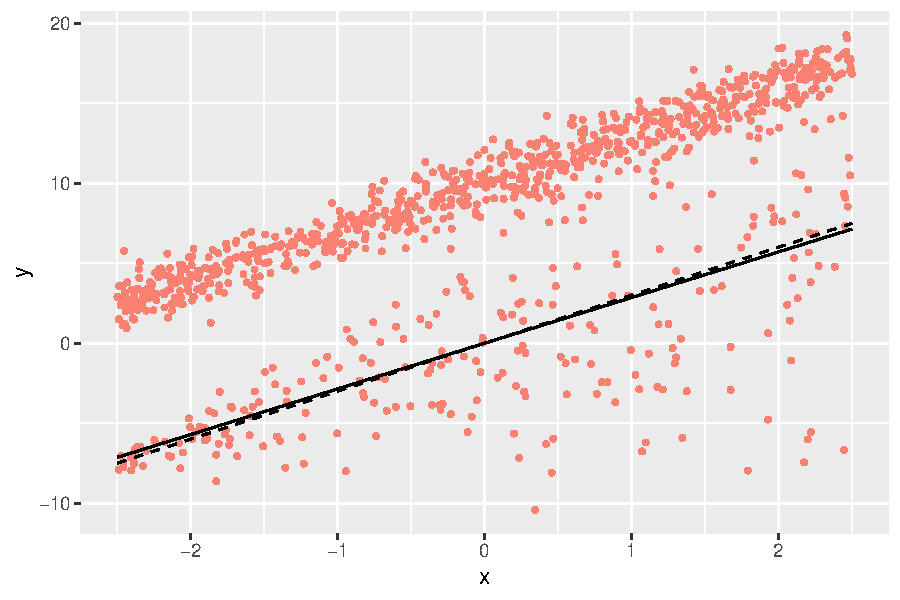
\includegraphics[width=.48\textwidth]{figures/fig1a} &
    \hskip-3pt
    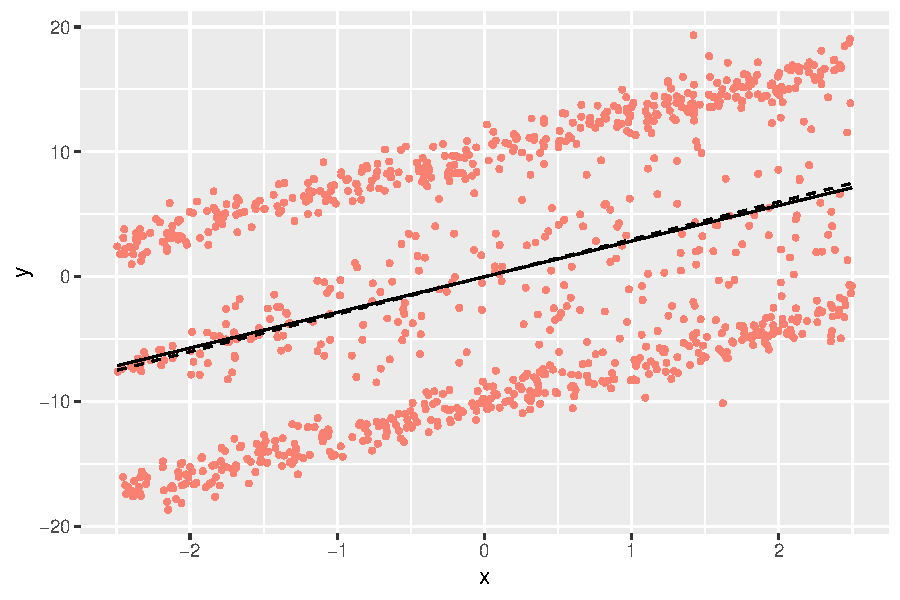
\includegraphics[width=.48\textwidth]{figures/fig1b}\\[-5pt]
  \end{tabular}
\caption{Median regression for corrupted data with $n=1{,}000$ and $\epsilon=0.75$.
The baseline noise is heteroskedastic, with distribution $P_i = N(0, (1.5 x_i + 4)^2)$
for data point $x_i$. Left: Corrupting distributions
$Q_i = N(10, 1)$. Right: Corrupting distributions $Q_i = N(10 \cdot W_i, 1)$ where $W_i$ are
independent Rademacher random variables. The solid line is the true regression
function, and the dashed line is the fit using median regression.}
\label{fig:exp}
\vskip20pt
  \begin{center}
    \begin{tabular}{cc}
      \hskip-10pt
      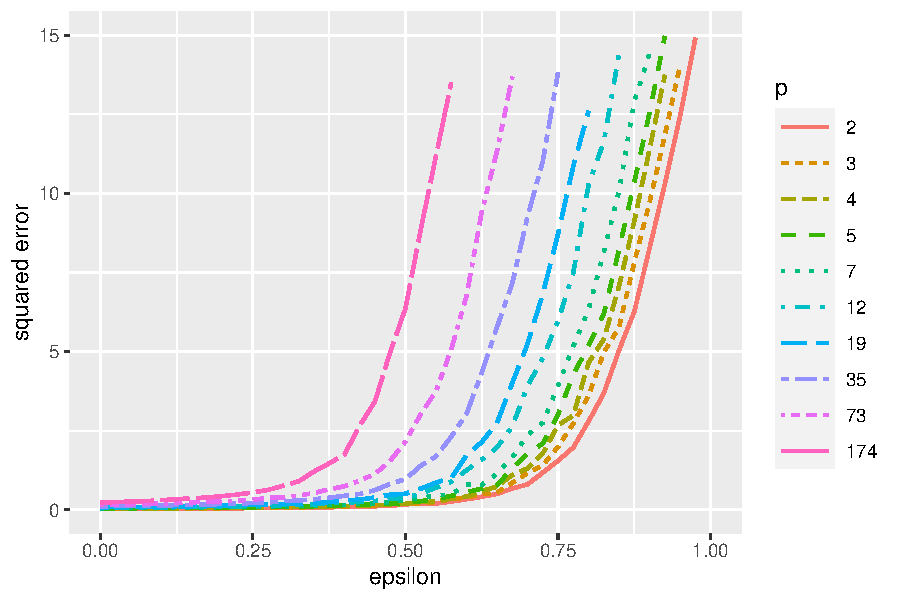
\includegraphics[width=.48\textwidth]{figures/fig2a}&
      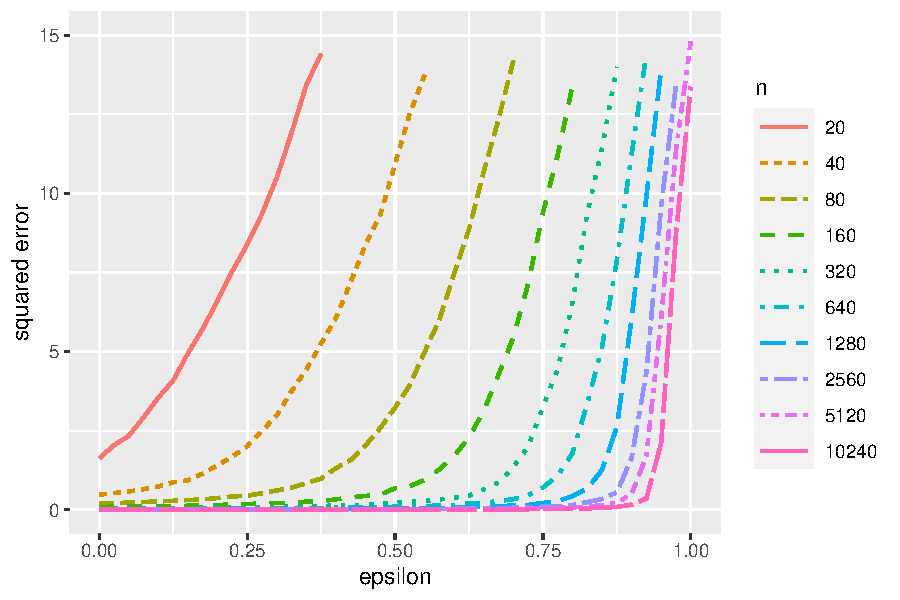
\includegraphics[width=.48\textwidth]{figures/fig2b}\\[-5pt]
    \end{tabular}
  \end{center}
\caption{Robust lasso for the linear model  $y=X\beta + z$ with design points $X_{ij}\sim N(0,1)$.
Left: Dimension $p$ varying as $p_{j} = e^{\rho^j}$, rounded down to the nearest integer, with $\rho=1.2$; the sample size is fixed at $n=100$, and $s=2$. Right: Dimension fixed at $p=10$ with $s=5$ relevant variables; the sample size $n$ is varied according to
$n_j = 2^j \cdot 20$ for $j=0,\ldots, 9$. The vertical axis shows the squared error $\|\hat \beta - \beta^*\|^2$ averaged over multiple trials.}
\end{figure*}

% !TEX root = ./robust.tex


\section{Proofs}
\label{sec:proofs}

\subsection{Some Technical Lemmas}

We first need a result that shows Condition A implies both high-probability and in-expectation bounds for $\left\|\frac{1}{n}\sum_{i=1}^nc_ix_i\right\|_{\infty}$.

\begin{lemma}\label{lem:random-part}
Suppose Condition A holds. Then, for any fixed (not random) $c_1,\cdots,c_n\in[-1,1]$, we have
\begin{equation}
\mathbb{P}\left(\left\|\frac{1}{n}\sum_{i=1}^nc_ix_i\right\|_{\infty}>t\right)\leq 2p\exp\left(-\frac{nt^2}{2\overline{\kappa}^2}\right), \label{eq:tail-inf}
\end{equation}
for any $t>0$. Moreover,
\begin{equation}
\mathbb{E}\left\|\frac{1}{n}\sum_{i=1}^nc_ix_i\right\|_{\infty} \leq \overline{\kappa}\sqrt{\frac{2\log(2p)}{n}}. \label{eq:exp-inf}
\end{equation}
\end{lemma}
\begin{proof}
For any $\rho\geq 0$, we have Chernoff's bound
$$\mathbb{P}\left(\left\|\frac{1}{n}\sum_{i=1}^nc_ix_i\right\|_{\infty}>t\right) \leq e^{-\rho t}\mathbb{E}\exp\left(\rho\left\|\frac{1}{n}\sum_{i=1}^nc_ix_i\right\|_{\infty}\right) \leq 2p\exp\left(-\rho t+\frac{\overline{\kappa}^2\rho^2}{2n}\right),$$
where we have used Condition A in the last inequality above. Optimizing over $\rho$, we obtain the bound (\ref{eq:tail-inf}) as desired. To get (\ref{eq:exp-inf}), we use Jensen's inequality and get
$$\mathbb{E}\left\|\frac{1}{n}\sum_{i=1}^nc_ix_i\right\|_{\infty} \leq \frac{1}{\rho}\log\mathbb{E}\exp\left(\rho\left\|\frac{1}{n}\sum_{i=1}^nc_ix_i\right\|_{\infty}\right) \leq \frac{1}{\rho}\log\left(2p\exp\left(\frac{\rho^2\overline{\kappa}^2}{2n}\right)\right).$$
Take $\rho=\sqrt{\frac{2n\log(2p)}{\overline{\kappa}^2}}$, and we obtain (\ref{eq:exp-inf}), which completes the proof.
\end{proof}


The next two lemmas are results in \cite{wang2013l1}.

\begin{lemma}\label{lem:link-to-loss}
Suppose Condition N holds. Then, we have
$$\mathbb{E}_{z\sim P_i}\left(|t+z|-|z|\right) \geq \frac{1}{16}|t|\left(\frac{|t|}{\sigma}\wedge 6\right),$$
for any $t>0$ and any $i\in[n]$.
\end{lemma}

\begin{lemma}
For any $v\in\mathbb{R}^n$, we have $\sum_{i=1}^n\left(|v_i|\wedge |v_i|^2\right)\geq \frac{\|v\|_1}{2}\wedge \|v\|^2$.
\end{lemma}

The following result is Theorem 4.12 of \cite{ledoux2013probability}.

\begin{lemma}\label{lem:contraction}
Let $F:\mathbb{R}_+\rightarrow\mathbb{R}_+$ be convex and increasing. Let further $\psi_i:\mathbb{R}\rightarrow\mathbb{R}$, $i\leq n$, be contractions such that $\psi(0)=0$. Then, for any bounded subset $T\subset\mathbb{R}^n$,
$$\mathbb{E}F\left(\frac{1}{2}\sup_{t\in T}\left|\sum_{i=1}^n\delta_i\psi_i(t_i)\right|\right)\leq \mathbb{E}F\left(\sup_{t\in T}\left|\sum_{i=1}^n\delta_i t_i\right|\right),$$
where $\delta_1,...,\delta_n$ are i.i.d. $\text{Unif}\{\pm 1\}$.
\end{lemma}


Finally, we need a result that establishes the conclusions of Lemma \ref{lem:random-part} under Condition A'.

\begin{lemma}\label{lem:random-heavy}
Suppose Condition A' is satisfied with some constant $\eta\geq 4$. Assume $n^{\frac{\eta-2}{2}}>p^{1.01}$. Then, for any fixed (not random) $c_1,\cdots,c_n\in[-1,1]$, we have
$$\mathbb{E}\left\|\frac{1}{n}\sum_{i=1}^nc_ix_i\right\|_{\infty} \leq 4\overline{\kappa}\sqrt{\frac{\log(2p)}{n}}.$$
Moreover, for any fixed (not random) $c_1,\cdots,c_n\in[-1,1]$ and any $t>0$, we also have
$$\left\|\frac{1}{n}\sum_{i=1}^nc_ix_i\right\|_{\infty}\leq 3\overline{\kappa}\sqrt{\frac{\log(2p)}{n}},$$
and
$$\mathbb{E}\left[\exp\left(t\left\|\sum_{i=1}^n\delta_ix_i\right\|_{\infty}\right)\Bigg|X\right]\leq 2p\exp\left(nt^2\overline{\kappa}^2\right),$$
with probability at least $1-p^{-0.009}$, where $\delta_1,...,\delta_n$ are i.i.d. $\text{Unif}\{\pm 1\}$.
\end{lemma}
\begin{proof}
We take $c_i=1$ for simplicity. The proof for general $\{c_i\}_{i\in[n]}$ follows the same argument. Define
\begin{eqnarray*}
\bar{x}_{ij} &=& x_{ij}\mathbb{I}\{|x_{ij}|\leq\tau\}-\mathbb{E}x_{ij}\mathbb{I}\{|x_{ij}|\leq\tau\}, \\
\wt{x}_{ij} &=& x_{ij}\mathbb{I}\{|x_{ij}|>\tau\}-\mathbb{E}x_{ij}\mathbb{I}\{|x_{ij}|>\tau\}.
\end{eqnarray*}
Then, we have the decomposition $x_{ij}=\bar{x}_{ij}+\wt{x}_{ij}$. For any $t>0$,
\begin{eqnarray*}
&& \mathbb{P}\left(\max_{j\in[p]}\left|\frac{1}{n}\sum_{i=1}^nx_{ij}\right|>\overline{\kappa} t\right) \\
&\leq& \mathbb{P}\left(\max_{j\in[p]}\left|\frac{1}{n}\sum_{i=1}^n\bar{x}_{ij}\right|>\overline{\kappa} t/2\right) + \mathbb{P}\left(\max_{j\in[p]}\left|\frac{1}{n}\sum_{i=1}^n\wt{x}_{ij}\right|>\overline{\kappa} t/2\right).
\end{eqnarray*}
For the first term, we use Bernstein's inequality and union bound, and get
\begin{equation}
\mathbb{P}\left(\max_{j\in[p]}\left|\frac{1}{n}\sum_{i=1}^n\bar{x}_{ij}\right|>\overline{\kappa} t/2\right)\leq 2p\exp\left(-\frac{n^2\overline{\kappa}^2t^2/4}{n\overline{\kappa}^2+n\overline{\kappa} t\tau/3}\right). \label{eq:ht-bern}
\end{equation}
Now we set $\tau=\overline{\kappa}\sqrt{\frac{n}{\log(2p)}}$ and $t=3\sqrt{\frac{\log(2p)}{n}}$. We can then conclude that
\begin{equation}
\max_{j\in[p]}\left|\frac{1}{n}\sum_{i=1}^n\bar{x}_{ij}\right|\leq \frac{3}{2}\overline{\kappa}\sqrt{\frac{\log p}{n}}, \label{eq:ht-01}
\end{equation}
with probability at least $1-(2p)^{-1/8}$. To analyze the second term, we note that
\begin{eqnarray}
\nonumber |\mathbb{E}x_{ij}\mathbb{I}\{|x_{ij}|>\tau\}|/\overline{\kappa} &\leq& \left(\mathbb{E}\left|\frac{x_{ij}}{\overline{\kappa}}\right|^{\eta}\right)^{1/\eta} \mathbb{P}\left(|x_{ij}|>\tau\right)^{\frac{\eta-1}{\eta}} \\
\nonumber &\leq&  \mathbb{P}\left(|x_{ij}|>\overline{\kappa}\sqrt{\frac{n}{\log(2p)}}\right)^{\frac{\eta-1}{\eta}} \\
\label{eq:holder-moment} &\leq& \left(\frac{\log (2p)}{n}\right)^{\frac{\eta-1}{2}},
\end{eqnarray}
where the last inequality is by Condition A'.
This implies $|\mathbb{E}x_{ij}\mathbb{I}\{|x_{ij}|>\tau\}|\leq \overline{\kappa}\left(\frac{\log (2p)}{n}\right)^{\frac{\eta-1}{2}}$.
Recall that we have set $t=3\sqrt{\frac{\log(2p)}{n}}$. As long as $\eta>2$ and $\frac{\log(2p)}{n}$ is sufficiently small so that $\left(\frac{\log(2p)}{n}\right)^{\frac{\eta-2}{2}}<\frac{3}{2}$ holds, we have
\begin{eqnarray*}
&& \mathbb{P}\left(\max_{j\in[p]}\left|\frac{1}{n}\sum_{i=1}^n\wt{x}_{ij}\right|>\overline{\kappa} t/2\right) \\
&\leq& \mathbb{P}\left(\max_{j\in[p]}\left|\frac{1}{n}\sum_{i=1}^nx_{ij}\mathbb{I}\{|x_{ij}|>\tau\}\right|>\overline{\kappa} t/4\right) \\
&\leq& \sum_{j=1}^p\sum_{i=1}^n\mathbb{P}(|x_{ij}|>\tau) \\
&\leq& pn \left(\frac{\log (2p)}{n}\right)^{\frac{\eta}{2}}.
\end{eqnarray*}
Therefore, under the condition $n^{\frac{\eta-2}{2}}>p^{1.01}$, we also have
\begin{equation}
\max_{j\in[p]}\left|\frac{1}{n}\sum_{i=1}^n\wt{x}_{ij}\right|\leq \frac{3}{2}\overline{\kappa}\sqrt{\frac{\log (2p)}{n}}, \label{eq:ht-02}
\end{equation}
with probability at least $1-p^{-0.009}$. We thus obtain the second conclusion by combining (\ref{eq:ht-01}) and (\ref{eq:ht-02}). For the first conclusion, we have
$$\mathbb{E}\max_{j\in[p]}\left|\frac{1}{n}\sum_{i=1}^n{x}_{ij}\right|/\overline{\kappa}\leq \mathbb{E}\max_{j\in[p]}\left|\frac{1}{n}\sum_{i=1}^n\bar{x}_{ij}\right|/\overline{\kappa}+\mathbb{E}\max_{j\in[p]}\left|\frac{1}{n}\sum_{i=1}^n\wt{x}_{ij}\right|/\overline{\kappa},$$
and we will bound the two terms on the right hand side of the above bound separately. The first term can be bounded by integrating up the tail bound (\ref{eq:ht-bern}) with $\tau=\overline{\kappa}\sqrt{\frac{n}{\log(2p)}}$. We have
\begin{eqnarray*}
\mathbb{E}\max_{j\in[p]}\left|\frac{1}{n}\sum_{i=1}^n\bar{x}_{ij}\right|/\overline{\kappa} &=& \int_0^{\infty}\mathbb{P}\left(\max_{j\in[p]}\left|\frac{1}{n}\sum_{i=1}^n\bar{x}_{ij}\right|>\overline{\kappa} t/2\right)dt \\
&\leq& 3\sqrt{\frac{\log (2p)}{n}} + \int_{3\sqrt{\frac{\log (2p)}{n}}}^{\infty}2p\exp\left(-\frac{nt^2}{8}\right)dt + \int_{3\sqrt{\frac{\log (2p)}{n}}}^{\infty}2p\exp\left(-\frac{n\overline{\kappa} t}{3\tau}\right)dt \\
&\leq& 4\sqrt{\frac{\log (2p)}{n}},
\end{eqnarray*}
and thus $\mathbb{E}\max_{j\in[p]}\left|\frac{1}{n}\sum_{i=1}^n\bar{x}_{ij}\right|\leq 4\overline{\kappa}\sqrt{\frac{\log (2p)}{n}}$. For the second term, we have
\begin{eqnarray*}
\mathbb{E}\max_{j\in[p]}\left|\frac{1}{n}\sum_{i=1}^n\wt{x}_{ij}\right|/\overline{\kappa} &\leq& \frac{2}{n}\sum_{j=1}^p\sum_{i=1}^n|\mathbb{E}x_{ij}\mathbb{I}\{|x_{ij}|>\tau\}|/\overline{\kappa} \\
&\leq& 2p\left(\frac{\log (2p)}{n}\right)^{\frac{\eta-1}{2}} \\
&\leq& \sqrt{\frac{\log (2p)}{n}},
\end{eqnarray*}
where the first inequality in the above display uses the same argument that leads to (\ref{eq:holder-moment}), and the second inequality holds under the condition $n^{\frac{\eta-2}{2}}>p^{1.01}$. Hence, we have $\mathbb{E}\max_{j\in[p]}\left|\frac{1}{n}\sum_{i=1}^n{x}_{ij}\right|/\overline{\kappa}\leq 5\sqrt{\frac{\log (2p)}{n}}$ and thus the first conclusion is proved.

For the last conclusion, we define $w_{ij}=x_{ij}^2$, and
\begin{eqnarray*}
\bar{w}_{ij} &=& w_{ij}\mathbb{I}\{|w_{ij}|\leq\tau\}-\mathbb{E}w_{ij}\mathbb{I}\{|w_{ij}|\leq\tau\}, \\
\wt{w}_{ij} &=& w_{ij}\mathbb{I}\{|w_{ij}|>\tau\}-\mathbb{E}w_{ij}\mathbb{I}\{|w_{ij}|>\tau\}.
\end{eqnarray*}
Then $w_{ij}=\bar{w}_{ij}+\wt{w}_{ij}$. By Bernstein's inequality and union bound, we have
$$\mathbb{P}\left(\max_{j\in[p]}\left|\frac{1}{n}\sum_{i=1}^n\bar{w}_{ij}\right|>\overline{\kappa}^2 t/2\right)\leq 2p\exp\left(-\frac{n^2\overline{\kappa}^4t^2/2}{n\overline{\kappa}^4+n\overline{\kappa}^2 t\tau/6}\right).$$
We choose $\tau=\frac{n\overline{\kappa}^2}{\log(2p)}$ and $t=1$. This implies $\max_{j\in[p]}\left|\frac{1}{n}\sum_{i=1}^n\bar{w}_{ij}\right|\leq \overline{\kappa}^2/2$ with probability at least $1-(2p)^{-5}$ as long as $\frac{\log(2p)}{n}<\frac{1}{6}$. To analyze the second term, we note that
\begin{eqnarray*}
|\mathbb{E}w_{ij}\mathbb{I}\{|w_{ij}|>\tau\}|/\overline{\kappa}^2 &\leq& \left(\mathbb{E}\left|\frac{w_{ij}}{\overline{\kappa}^2}\right|^{\eta/2}\right)^{2/\eta} \mathbb{P}\left(|w_{ij}|>\tau\right)^{\frac{\eta-2}{\eta}} \\
&\leq&  \mathbb{P}\left(|w_{ij}|>\tau\right)^{\frac{\eta-2}{\eta}} \\
&\leq& \left(\frac{\log (2p)}{n}\right)^{\frac{\eta-2}{2}}.
\end{eqnarray*}
Therefore, for $\frac{\log (2p)}{n}$ that is sufficiently small, we have
\begin{eqnarray*}
&& \mathbb{P}\left(\max_{j\in[p]}\left|\frac{1}{n}\sum_{i=1}^n\wt{w}_{ij}\right|>\overline{\kappa}^2/2\right) \\
&\leq& \mathbb{P}\left(\max_{j\in[p]}\left|\frac{1}{n}\sum_{i=1}^nw_{ij}\mathbb{I}\{|w_{ij}|>\tau\}\right|>\overline{\kappa}/4\right) \\
&\leq& \sum_{j=1}^p\sum_{i=1}^n\mathbb{P}(|w_{ij}|>\tau) \\
&\leq& pn \left(\frac{\log (2p)}{n}\right)^{\frac{\eta}{2}}.
\end{eqnarray*}
Under the condition $n^{\frac{\eta-2}{2}}>p^{1.01}$, we also have $\max_{j\in[p]}\left|\frac{1}{n}\sum_{i=1}^n\wt{w}_{ij}\right|\leq \overline{\kappa}^2/2$ with probability at least $1-p^{-0.009}$. We can conclude that
\begin{equation}
\max_{j\in[p]}\sum_{i=1}^nx_{ij}^2\leq \overline{\kappa}^2n,\label{eq:nice-x}
\end{equation}
with probability at least $1-p^{-0.009}$. Whenever (\ref{eq:nice-x}) holds, we have
\begin{eqnarray*}
\mathbb{E}\left[\exp\left(t\left\|\sum_{i=1}^n\delta_ix_i\right\|_{\infty}\right)\Bigg|X\right] &\leq& \sum_{j=1}^p\mathbb{E}\left[\exp\left(t\left|\sum_{i=1}^n\delta_ix_{ij}\right|\right)\Bigg|X\right] \\
&\leq& \sum_{j=1}^p\mathbb{E}\left[\exp\left(t\sum_{i=1}^n\delta_ix_{ij}\right)\Bigg|X\right] + \sum_{j=1}^p\mathbb{E}\left[\exp\left(-t\sum_{i=1}^n\delta_ix_{ij}\right)\Bigg|X\right] \\
&=& 2\sum_{j=1}^p\prod_{i=1}^n\mathbb{E}\left(e^{t\delta_ix_{ij}}\Big|X\right) \\
&=& 2\sum_{j=1}^p\prod_{i=1}^n\left(\frac{1}{2}e^{tx_{ij}}+\frac{1}{2}e^{-tx_{ij}}\right) \\
&\leq& 2\sum_{j=1}^p\exp\left(t^2\sum_{i=1}^nx_{ij}^2\right) \\
&\leq& 2p\exp\left(nt^2\overline{\kappa}^2\right).
\end{eqnarray*}
This completes the proof.
\end{proof}


\subsection{Proofs of Theorem \ref{thm:main} and Theorem \ref{thm:heavy}}

\begin{proof}[Proof of Theorem \ref{thm:main}]
Define $L_n(\beta)=\frac{1}{n}\sum_{i=1}^n\left(|x_i^T(\beta^*-\beta)+z_i|-|z_i|\right)$, and $L(\beta)=\mathbb{E}L_n(\beta)$, where the expectation is over the joint distribution of design and noise. It is easy to see that $L_n(\beta^*)=0$. We introduce the notation
$$\ell_{\Sigma}(\beta,\beta^*)=\frac{1}{n}\sum_{i=1}^n\|\Sigma_i^{1/2}(\beta-\beta^*)\|.$$
Now suppose $\ell_{\Sigma}(\wh{\beta},\beta^*)\geq \underline{\kappa}t$, we have
$$\inf_{\ell_{\Sigma}(\beta,\beta^*)\geq\underline{\kappa}t}(L_n(\beta)+\lambda\|\beta\|_1)\leq L_n(\beta^*)+\lambda\|\beta^*\|_1=\lambda\|\beta^*\|_1.$$
By the convexity of $L_n(\beta)+\lambda\|\beta\|_1$, we can replace $\ell_{\Sigma}(\beta,\beta^*)\geq\underline{\kappa}t$ with $\ell_{\Sigma}(\beta,\beta^*)=\underline{\kappa}t$. Then,
\begin{equation}
\inf_{\ell_{\Sigma}(\beta,\beta^*)=\underline{\kappa}t}(L_n(\beta)+\lambda\|\beta\|_1-\lambda\|\beta^*\|_1)\leq 0. \label{eq:basic}
\end{equation}

\paragraph{Cone Condition.}
Since $L_n(\beta)$ is a convex function, we have
$$L_n(\beta)\geq L_n(\beta^*)+\nabla L_n(\beta^*)^T(\beta-\beta^*).$$
Therefore,
\begin{eqnarray*}
&& L_n(\beta)+\lambda\|\beta\|_1-\lambda\|\beta^*\|_1 \\
&\geq& \frac{1}{n}\sum_{i=1}^n\sgn(z_i)x_i^T(\beta^*-\beta)+\lambda\|\beta\|_1-\lambda\|\beta^*\|_1 \\
&\geq& -\left\|\frac{1}{n}\sum_{i=1}^n\sgn(z_i)x_i\right\|_{\infty}\|\beta-\beta^*\|_1+\lambda\|\beta\|_1-\lambda\|\beta^*\|_1  \\
&\geq& \left(\lambda-\left\|\frac{1}{n}\sum_{i=1}^n\sgn(z_i)x_i\right\|_{\infty}\right)\|(\beta-\beta^*)_{S^c}\|_1 - \left(\lambda+\left\|\frac{1}{n}\sum_{i=1}^n\sgn(z_i)x_i\right\|_{\infty}\right)\|(\beta-\beta^*)_{S}\|_1.
\end{eqnarray*}
As long as $\lambda\geq 2\left\|\frac{1}{n}\sum_{i=1}^n\sgn(z_i)x_i\right\|_{\infty}$, we have
$$L_n(\beta)+\lambda\|\beta\|_1-\lambda\|\beta^*\|_1 \geq \frac{\lambda}{2}\|(\beta-\beta^*)_{S^c}\|_1-\frac{3\lambda}{2}\|(\beta-\beta^*)_{S}\|_1,$$
where $S=\{j\in[p]:\beta_j^*\neq 0\}$.
For any $\beta$ such that $L_n(\beta)+\lambda\|\beta\|_1-\lambda\|\beta^*\|_1\leq 0$ holds, we must have $0\geq \frac{\lambda}{2}\|(\beta-\beta^*)_{S^c}\|_1-\frac{3\lambda}{2}\|(\beta-\beta^*)_{S}\|_1,$
which implies the cone condition
\begin{equation}
\|(\beta-\beta^*)_{S^c}\|_1\leq 3\|(\beta-\beta^*)_{S}\|_1.\label{eq:cone}
\end{equation}
Define $\mathcal{C}$ to be the collection of $\beta$ such that (\ref{eq:cone}) is satisfied. We have shown that $L_n(\beta)+\lambda\|\beta\|_1-\lambda\|\beta^*\|_1\leq 0$ implies $\beta\in\mathcal{C}$. Therefore, we can add the additional constraint $\mathcal{C}$ to the inequality (\ref{eq:basic}), and we thus obtain
\begin{equation}
\inf_{\beta\in\mathcal{C}:\ell_{\Sigma}(\beta,\beta^*)=\underline{\kappa}t}(L_n(\beta)+\lambda\|\beta\|_1-\lambda\|\beta^*\|_1)\leq 0, \label{eq:basic-cone}
\end{equation}
whenever $\lambda\geq 2\left\|\frac{1}{n}\sum_{i=1}^n\sgn(z_i)x_i\right\|_{\infty}$ holds.
By Lemma \ref{lem:random-part}, we have $\lambda\geq 2\left\|\frac{1}{n}\sum_{i=1}^n\sgn(z_i)x_i\right\|_{\infty}$ with probability at least $1-(2p)^{-1/8}$ with the choice $\lambda=3\overline{\kappa}\sqrt{\frac{\log(2p)}{n}}$. This implies (\ref{eq:basic-cone}) holds with probability at least $1-(2p)^{-1/8}$.

\paragraph{Stochastic Error.}
From (\ref{eq:basic-cone}), we can derive
\begin{eqnarray*}
&& \inf_{\beta\in\mathcal{C}:\ell_{\Sigma}(\beta,\beta^*)=\underline{\kappa}t}(L(\beta)+\lambda\|\beta\|_1-\lambda\|\beta^*\|_1) \\
&\leq& \inf_{\beta\in\mathcal{C}:\ell_{\Sigma}(\beta,\beta^*)=\underline{\kappa}t}(L_n(\beta)+\lambda\|\beta\|_1-\lambda\|\beta^*\|_1) + \sup_{\beta\in\mathcal{C}:\ell_{\Sigma}(\beta,\beta^*)=\underline{\kappa}t}(L(\beta)-L_n(\beta)) \\
&\leq& \sup_{\beta\in\mathcal{C}:\ell_{\Sigma}(\beta,\beta^*)=\underline{\kappa}t}(L(\beta)-L_n(\beta)).
\end{eqnarray*}
We thus need to give a bound for $\sup_{\beta\in\mathcal{C}:\ell_{\Sigma}(\beta,\beta^*)=\underline{\kappa}t}(L(\beta)-L_n(\beta))$. For any $\beta\in\mathcal{C}$ that satisfies $\ell_{\Sigma}(\beta,\beta^*)=\underline{\kappa}t$, we have
\begin{eqnarray}
\nonumber \|\beta-\beta^*\|_1 &=& \|(\beta-\beta^*)_{S^c}\|_1 + \|(\beta-\beta^*)_{S}\|_1 \\
\nonumber &\leq& 4\|(\beta-\beta^*)_{S}\|_1 \\
\nonumber &\leq& 4\sqrt{s}\|\beta-\beta^*\| \\
\label{eq:bound-for-l1} &\leq& \frac{4\sqrt{s}}{\underline{\kappa}}\ell_{\Sigma}(\beta,\beta^*) \leq 4\sqrt{s}t.
\end{eqnarray}
Therefore,
$$\sup_{\beta\in\mathcal{C}:\ell_{\Sigma}(\beta,\beta^*)=\underline{\kappa}t}(L(\beta)-L_n(\beta))\leq \sup_{\|\beta-\beta^*\|_1\leq 4\sqrt{s}t}(L(\beta)-L_n(\beta)).$$
We use $\mathbb{E}^X$ for the conditional expectation operator $\mathbb{E}(\cdot|X)$. Then, a standard symmetrization argument (Lemma 2.3.1 of \cite{wellner2013weak}) leads to
\begin{eqnarray*}
&& \mathbb{E}^X\exp\left(\rho \sup_{\|\beta-\beta^*\|_1\leq 4\sqrt{s}t}(L(\beta)-L_n(\beta))\right) \\
&\leq& \mathbb{E}^X\exp\left(2\rho \sup_{\|\beta-\beta^*\|_1\leq 4\sqrt{s}t}\left|\frac{1}{n}\sum_{i=1}^n\delta_i\left(|x_i^T(\beta^*-\beta)+z_i|-|z_i|\right)\right|\right),
\end{eqnarray*}
for any $\rho>0$, where $\delta_1,\cdots,\delta_n$ are i.i.d. $\text{Unif}\{\pm 1\}$. Use Lemma \ref{lem:contraction}, and the above quantity can be further bounded by
\begin{eqnarray*}
&& \mathbb{E}^X\exp\left(4\rho\sup_{\|\beta-\beta^*\|_1\leq 4\sqrt{s}t}\left|\frac{1}{n}\sum_{i=1}^n\delta_ix_i^T(\beta-\beta^*)\right|\right) \\
&\leq& \mathbb{E}^X\exp\left(16\rho\sqrt{s}t \left\|\frac{1}{n}\sum_{i=1}^n\delta_ix_i\right\|_{\infty}\right).
\end{eqnarray*}
We have thus obtained the bound
\begin{equation}
\mathbb{E}^X\exp\left(\rho \sup_{\|\beta-\beta^*\|_1\leq 4\sqrt{s}t}(L(\beta)-L_n(\beta))\right)\leq  \mathbb{E}^X\exp\left(16\rho\sqrt{s}t \left\|\frac{1}{n}\sum_{i=1}^n\delta_ix_i\right\|_{\infty}\right). \label{eq:cond-mgf}
\end{equation}
Taking expectation on both sides, we then have
$$\mathbb{E}\exp\left(\rho \sup_{\|\beta-\beta^*\|_1\leq 4\sqrt{s}t}(L(\beta)-L_n(\beta))\right)\leq \mathbb{E}\exp\left(16\rho\sqrt{s}t \left\|\frac{1}{n}\sum_{i=1}^n\delta_ix_i\right\|_{\infty}\right).$$
By Condition A, the right hand side of the above inequality can be bounded by $2p\exp\left(128\rho^2s t^2\overline{\kappa}^2/n\right)$. By Chernoff bound, we have
$$\mathbb{P}\left(\sup_{\|\beta-\beta^*\|_1\leq 4\sqrt{s}t}(L(\beta)-L_n(\beta)) > x\right)\leq 2p\exp\left(128\rho^2s t^2\overline{\kappa}^2/n-\rho x\right).$$
Optimize over $\rho$, and we get
$$\mathbb{P}\left(\sup_{\|\beta-\beta^*\|_1\leq 4\sqrt{s}t}(L(\beta)-L_n(\beta)) > x\right)\leq 2p\exp\left(-\frac{nx^2}{512st^2\overline{\kappa}^2}\right),$$
which implies
$$\sup_{\|\beta-\beta^*\|_1\leq 4\sqrt{s}t}(L(\beta)-L_n(\beta))\leq 24t\overline{\kappa}\sqrt{\frac{s\log (2p)}{n}},$$
with probability at least $1-(2p)^{-1/8}$.
To summarize, we have established that
\begin{equation}
\inf_{\beta\in\mathcal{C}:\ell_{\Sigma}(\beta,\beta^*)=\underline{\kappa}t}(L(\beta)+\lambda\|\beta\|_1-\lambda\|\beta^*\|_1) \leq 24t\overline{\kappa}\sqrt{\frac{s\log (2p)}{n}}, \label{eq:pf-main-l}
\end{equation}
with probability at least $1-2(2p)^{-1/8}$.

\paragraph{Identifiability.} For any $\beta\in\mathcal{C}$ that satisfies $\ell_{\Sigma}(\beta,\beta^*)=\underline{\kappa}t$, we need to find a lower bound for $L(\beta)+\lambda\|\beta\|_1-\lambda\|\beta^*\|_1$.
We first give a lower bound for $\lambda\|\beta\|_1-\lambda\|\beta^*\|_1$, and we have
\begin{equation}
\lambda\|\beta\|_1-\lambda\|\beta^*\|_1\geq -\lambda\|\beta-\beta^*\|_1 \geq -4\sqrt{s}\lambda t, \label{eq:pen-easy}
\end{equation}
where the last inequality has been established in (\ref{eq:bound-for-l1}).
Next, we analyze $L(\beta)$.
Define $f_i(x)=\mathbb{E}_{z_i\sim Q_i}(|x+z_i|-|z_i|)$ and $Q_i(x)=Q_i(z_i\leq x)$. It is easy to check that $f_i(0)=0$ and $f_i'(x)=1-2Q_i(x)$. Then, by convexity, we have
\begin{eqnarray*}
\frac{1}{n}\sum_{i=1}^nf_i(x_i^T(\beta^*-\beta)) &\geq& \frac{1}{n}\sum_{i=1}^nf_i(0) + \frac{1}{n}\sum_{i=1}^nf_i'(0)x_i^T(\beta^*-\beta) \\
&=& \frac{1}{n}\sum_{i=1}^n(1-2Q_i(0))x_i^T(\beta^*-\beta) \\
&\geq& -4\sqrt{s}t\left\|\frac{1}{n}\sum_{i=1}^n(1-2Q_i(0))x_i\right\|_{\infty}.
\end{eqnarray*}
Lemma \ref{lem:random-part} implies that $\mathbb{E}\left\|\frac{1}{n}\sum_{i=1}^n(1-2Q_i(0))x_i\right\|_{\infty}\leq \overline{\kappa}\sqrt{\frac{2\log(2p)}{n}}$. Therefore,
$$\frac{1}{n}\sum_{i=1}^n\mathbb{E}f_i(x_i^T(\beta^*-\beta))\geq -4t\overline{\kappa}\sqrt{\frac{2s\log(2p)}{n}}.$$
Let us also define $g_i(x)=\mathbb{E}_{z_i\sim P_i}(|x+z_i|-|z_i|)$. By Lemma \ref{lem:link-to-loss}, we have $g_i(x)\geq \frac{1}{16}|x|\left(\frac{|x|}{\sigma}\wedge 6\right)$. Thus,
$$\frac{1}{n}\sum_{i=1}^n\mathbb{E}g_i(x_i^T(\beta^*-\beta))\geq \frac{1}{16n}\sum_{i=1}^n \mathbb{E}\left(\frac{|x_i^T(\beta^*-\beta)|^2}{\sigma}\wedge (6|x_i^T(\beta^*-\beta)|)\right).$$
For each $i\in[n]$, we have
\begin{align}
\nonumber & \mathbb{E}\left(\frac{|x_i^T(\beta^*-\beta)|^2}{\sigma}\wedge (6|x_i^T(\beta^*-\beta)|)\right) \\
\nonumber &= \mathbb{E}\frac{|x_i^T(\beta^*-\beta)|^2}{\sigma}\mathbb{I}\{|x_i^T(\beta^*-\beta)|< 6\sigma\} + 6\mathbb{E}|x_i^T(\beta^*-\beta)|\mathbb{I}\{|x_i^T(\beta^*-\beta)|\geq 6\sigma\} \\
\nonumber &\geq \mathbb{E}\frac{|x_i^T(\beta^*-\beta)|^2}{\sigma}\mathbb{I}\left\{\|\Sigma_i^{1/2}(\beta-\beta^*)\|< 6\sigma, \frac{|x_i^T(\beta^*-\beta)|^2}{\|\Sigma_i^{1/2}(\beta-\beta^*)\|^2}< 1\right\} \\
\nonumber & + 6\mathbb{E}|x_i^T(\beta^*-\beta)|\mathbb{I}\left\{\|\Sigma_i^{1/2}(\beta-\beta^*)\|\geq 6\sigma, \frac{|x_i^T(\beta^*-\beta)|^2}{\|\Sigma_i^{1/2}(\beta-\beta^*)\|^2}\geq 1\right\}  \\
\nonumber &= \frac{\|\Sigma_i^{1/2}(\beta-\beta^*)\|^2}{\sigma}\mathbb{I}\{\|\Sigma_i^{1/2}(\beta-\beta^*)\|< 6\sigma\}\mathbb{E}\frac{|x_i^T(\beta^*-\beta)|^2}{\|\Sigma_i^{1/2}(\beta-\beta^*)\|^2}\mathbb{I}\left\{\frac{|x_i^T(\beta^*-\beta)|^2}{\|\Sigma_i^{1/2}(\beta-\beta^*)\|^2}< 1\right\} \\
\nonumber & + 6\|\Sigma_i^{1/2}(\beta-\beta^*)\|\mathbb{I}\{\|\Sigma_i^{1/2}(\beta-\beta^*)\|\geq 6\sigma\}\mathbb{E}\frac{|x_i^T(\beta^*-\beta)|}{\|\Sigma_i^{1/2}(\beta-\beta^*)\|}\mathbb{I}\left\{\frac{|x_i^T(\beta^*-\beta)|^2}{\|\Sigma_i^{1/2}(\beta-\beta^*)\|^2}\geq 1\right\} \\
\label{eq:use-B} &\geq \frac{\|\Sigma_i^{1/2}(\beta-\beta^*)\|^2}{10\sigma}\mathbb{I}\{\|\Sigma_i^{1/2}(\beta-\beta^*)\|< 6\sigma\} + 6\|\Sigma_i^{1/2}(\beta-\beta^*)\|\mathbb{I}\{\|\Sigma_i^{1/2}(\beta-\beta^*)\|\geq 6\sigma\} \\
\nonumber &\geq \frac{\|\Sigma_i^{1/2}(\beta-\beta^*)\|^2}{10\sigma}\wedge\left(6\|\Sigma_i^{1/2}(\beta-\beta^*)\|\right),
\end{align}
where the inequality (\ref{eq:use-B}) is by Condition B.
Hence,
\begin{eqnarray}
\nonumber && \frac{1}{n}\sum_{i=1}^n\mathbb{E}g_i(x_i^T(\beta^*-\beta)) \\
\nonumber &\geq& \frac{1}{16n}\sum_{i=1}^n\left(\frac{\|\Sigma_i^{1/2}(\beta-\beta^*)\|^2}{10\sigma}\wedge\left(6\|\Sigma_i^{1/2}(\beta-\beta^*)\|\right)\right) \\
\nonumber &=&  \frac{45\sigma}{2n}\sum_{i=1}^n\left(\frac{\|\Sigma_i^{1/2}(\beta-\beta^*)\|^2}{(60\sigma)^2}\wedge \frac{\|\Sigma_i^{1/2}(\beta-\beta^*)\|}{60\sigma}\right) \\
\label{eq:use-wang} &\geq& \left(\frac{3}{16n}\sum_{i=1}^n\|\Sigma_i^{1/2}(\beta-\beta^*)\|\right) \wedge \left(\frac{1}{160n\sigma}\sum_{i=1}^n\|\Sigma_i^{1/2}(\beta-\beta^*)\|^2\right) \\
\nonumber &\geq& \left(\frac{3}{16n}\sum_{i=1}^n\|\Sigma_i^{1/2}(\beta-\beta^*)\|\right)\wedge \left(\frac{1}{160\sigma}\left[\frac{1}{n}\sum_{i=1}^n\|\Sigma_i^{1/2}(\beta-\beta^*)\|\right]^2\right) \\
\nonumber &=& \frac{3\underline{\kappa}t}{16}\wedge\frac{\underline{\kappa}^2t^2}{160\sigma}.
\end{eqnarray}
The inequality (\ref{eq:use-wang}) is by Lemma \ref{eq:use-wang}.
Combining the above bounds for $\frac{1}{n}\sum_{i=1}^n\mathbb{E}g_i(x_i^T(\beta^*-\beta))$ and $\frac{1}{n}\sum_{i=1}^n\mathbb{E}f_i(x_i^T(\beta^*-\beta))$, we obtain
\begin{eqnarray*}
L(\beta) &=& (1-\epsilon)\frac{1}{n}\sum_{i=1}^n\mathbb{E}g_i(x_i^T(\beta^*-\beta)) + \epsilon \frac{1}{n}\sum_{i=1}^n\mathbb{E}f_i(x_i^T(\beta^*-\beta)) \\
&\geq& (1-\epsilon)\left(\frac{3\underline{\kappa}t}{16}\wedge\frac{\underline{\kappa}^2t^2}{160\sigma}\right) -4\epsilon t\overline{\kappa}\sqrt{\frac{2s\log(2p)}{n}}.
\end{eqnarray*}
Together with (\ref{eq:pen-easy}), we have established that
\begin{eqnarray}
\nonumber && \inf_{\beta\in\mathcal{C}:\ell_{\Sigma}(\beta,\beta^*)=\underline{\kappa}t}(L(\beta)+\lambda\|\beta\|_1-\lambda\|\beta^*\|_1) \\
\label{eq:pf-main-u} &\geq& (1-\epsilon)\left(\frac{3\underline{\kappa}t}{16}\wedge\frac{\underline{\kappa}^2t^2}{160\sigma}\right) -4\epsilon t\overline{\kappa}\sqrt{\frac{2s\log(2p)}{n}} -4\sqrt{s}\lambda t.
\end{eqnarray}

\paragraph{Combine (\ref{eq:pf-main-l}) and (\ref{eq:pf-main-u}).} We shall combine (\ref{eq:pf-main-l}) and (\ref{eq:pf-main-u}), and then have the inequality
$$(1-\epsilon)\left(\frac{3\underline{\kappa}t}{16}\wedge\frac{\underline{\kappa}^2t^2}{160\sigma}\right) -4\epsilon t\overline{\kappa}\sqrt{\frac{2s\log(2p)}{n}} -4\sqrt{s}\lambda t\leq 24t\overline{\kappa}\sqrt{\frac{s\log (2p)}{n}},$$
with probability at least $1-2(2p)^{-1/8}$. With the choice $\lambda=3\overline{\kappa}\sqrt{\frac{\log(2p)}{n}}$, the above inequality can be rearranged into
\begin{equation}
\frac{3}{16}\wedge\frac{\underline{\kappa}t}{160\sigma}\leq 42\frac{\overline{\kappa}/\underline{\kappa}}{1-\epsilon}\sqrt{\frac{s\log(2p)}{n}}. \label{eq:make-contra}
\end{equation}
Under the condition $42\frac{\overline{\kappa}/\underline{\kappa}}{1-\epsilon}\sqrt{\frac{s\log(2p)}{n}}<\frac{3}{16}$, we can then choose $t$ that satisfies
$$\frac{\underline{\kappa}t}{160\sigma}=43\frac{\overline{\kappa}/\underline{\kappa}}{1-\epsilon}\sqrt{\frac{s\log(2p)}{n}}.$$
This makes the inequality (\ref{eq:make-contra}) impossible, and thus $\ell_{\Sigma}(\wh{\beta},\beta^*)\geq \underline{\kappa}t$ cannot hold. Hence, we have established that
$$\ell_{\Sigma}(\wh{\beta},\beta^*)\leq 6880 \frac{\overline{\kappa}/\underline{\kappa}}{1-\epsilon}\sqrt{\frac{\sigma^2s\log(2p)}{n}},$$
with probability at least $1-2(2p)^{-1/8}$. Finally, by $\|\wh{\beta}-\beta^*\|\leq \frac{1}{\underline{\kappa}}\ell_{\Sigma}(\wh{\beta},\beta^*)$, we also obtain the desired bound for $\|\wh{\beta}-\beta^*\|$.
\end{proof}


\begin{proof}[Proof of Theorem \ref{thm:heavy}]
The proof of Theorem \ref{thm:heavy} largely follows that of Theorem \ref{thm:main}, and we only list the differences of the two arguments. In establishing the cone condition, it is required to choose a $\lambda$ that satisfies  $\lambda\geq 2\left\|\frac{1}{n}\sum_{i=1}^n\sgn(z_i)x_i\right\|_{\infty}$ with high probability. By Lemma \ref{lem:random-heavy}, $\left\|\frac{1}{n}\sum_{i=1}^n\sgn(z_i)x_i\right\|_{\infty}\leq 3\overline{\kappa}\sqrt{\frac{\log(2p)}{n}}$ with high probability, and thus the choice $\lambda=6\overline{\kappa}\sqrt{\frac{\log(2p)}{n}}$ satisfied the requirement. When analyzing the stochastic error, we need to derive a high-probability bound for $\sup_{\|\beta-\beta^*\|_1\leq 4\sqrt{s}t}(L(\beta)-L_n(\beta))$. Use $\mathbb{E}^X$ and $\mathbb{P}^X$ for the conditional expectation and probability operators $\mathbb{E}(\cdot|X)$ and $\mathbb{P}(\cdot|X)$. By (\ref{eq:cond-mgf}) and Lemma \ref{lem:random-heavy}, we have
$$\mathbb{E}^X\exp\left(\rho \sup_{\|\beta-\beta^*\|_1\leq 4\sqrt{s}t}(L(\beta)-L_n(\beta))\right)\leq 2p\exp\left(\frac{256\overline{\kappa}^2\rho^2st^2}{n}\right),$$
for any $\rho>0$ with high probability. By a standard Chernoff bound argument, we have
$$\mathbb{P}^X\left(\sup_{\|\beta-\beta^*\|_1\leq 4\sqrt{s}t}(L(\beta)-L_n(\beta)) > x\right)\leq 2p\exp\left(-\frac{nx^2}{1024st^2\overline{\kappa}^2}\right),$$
with probability at least $1-p^{-0.009}$. Thus,
$$\sup_{\|\beta-\beta^*\|_1\leq 4\sqrt{s}t}(L(\beta)-L_n(\beta))\leq 48t\overline{\kappa}\sqrt{\frac{s\log (2p)}{n}},$$
with probability at least $1-(2p)^{-1/8}-p^{-0.009}$. Finally, in the identifiability analysis, we need to bound $\mathbb{E}\left\|\frac{1}{n}\sum_{i=1}^n(1-2Q_i(0))x_i\right\|_{\infty}$. Lemma \ref{lem:random-heavy} directly gives the bound
$$\mathbb{E}\left\|\frac{1}{n}\sum_{i=1}^n(1-2Q_i(0))x_i\right\|_{\infty}\leq 4\overline{\kappa}\sqrt{\frac{\log(2p)}{n}}.$$
The rest of the arguments are the same as in the proof of Theorem \ref{thm:main}.
\end{proof}

% !TEX root = ./robust.tex

\def\ones{{\mathds{1}}}

\section{Discussion}
\label{sec:discuss}


Compared with well-known Lasso error rates \citep{bickel2009simultaneous} $\sqrt{{s\log(p)}/{n}}$, our result shows an error rate $\frac{1}{1-\epsilon}\sqrt{{s\log(p)}/{n}}$ when the noise variables are contaminated. That is, the effective sample size is reduced to $n(1-\epsilon)^2$ from $n$. A natural question is whether the additional factor $(1-\epsilon)^2$ is optimal under the setting of robust linear regression with contaminated noise.

We give a partial answer to this question by studying a noiseless version of the problem. For the regression model $y_i=x_i^T\beta^*+z_i$, let us assume $z_i\sim (1-\epsilon)\delta_0 +\epsilon Q_i$ and the noise variables are independent from the design matrix. To recover $\beta^*$, we find $\wh{\beta}\in\mathcal{B}$, where
$$\mathcal{B}=\{\beta\in\mathbb{R}^p: y_i=x_i^T\beta\text{ for all }i\in\mathcal{N}\text{ with some }\mathcal{N}\subset[n]\text{ such that }|\mathcal{N}|\geq p+1\}.$$

\begin{condd}
For any $i_1,\cdots,i_{p+1}$, the conditional distribution of $x_{i_{p+1}}|x_{i_1},\cdots,x_{i_{p}}$ is non-degenerate.
\end{condd}

\begin{thm}\label{eq:noiseless}
Suppose Condition D holds. For any $\delta\in(0,1)$, there exists some $C>1$ only depending on $\delta$, such that whenever
$$\frac{n(1-\epsilon)}{p}>C,$$
we must have with probability at least $1-\delta$, the estimator $\wh{\beta}$ exists and satisfies $\wh{\beta}=\beta^*$.
\end{thm}
\begin{proof}
Note that the quantity $\sum_{i=1}^n\mathbb{I}\{z_i=0\}$ is stochastically greater than or equal to $\text{Binomial}(n,1-\epsilon)$. Under the condition that $n(1-\epsilon)>Cp$ for some sufficiently large $C$, we have
$$\mathbb{P}\left(\sum_{i=1}^n\mathbb{I}\{z_i=0\}\geq p+1\right)\geq \mathbb{P}\left(\text{Binomial}(n,1-\epsilon)\geq p+1\right)\geq 1-\delta.$$
In other words, there are at least $p+1$ observations with zero noise, which implies $y_i=x_i^T\beta^*$ for all $i$ in some subset of cardinality of $p+1$. Thus, the set $\mathcal{B}$ is not empty and $\wh{\beta}$ is well defined.

Now we show that $\mathcal{B}=\{\beta^*\}$. Suppose there exists some $\eta\in\mathcal{B}$. This means there exists some $\mathcal{N}$ with cardinality $p+1$ such that $y_i=x_i^T\eta$ for all $i\in\mathcal{N}$. Without loss of generality, let us write $\mathcal{N}=\{1,2,\cdots,p+1\}$ for simplicity of notation. Since $y_i=x_i^T\beta^*+z_i$ for all $i\in\mathcal{N}$, we have $x_i^T(\eta-\beta^*)=z_i$ for all $i\in\mathcal{N}$. These $p+1$ equations can be organized as $X(\eta-\beta^*)=z$ and $x_{p+1}^T(\eta-\beta^*)=z_{p+1}$, where $X$ is a $p\times p$ matrix with its $i$th row being $x_i^T$ and $z$ is a $p$-dimensional vector with its $i$th entry being $z_i$. Condition N implies that $X$ is invertible so that $\eta-\beta^*=X^{-1}z$, and thus $x_{p+1}^TX^{-1}z=z_{p+1}$. Conditioning on some $z\neq 0$ and some $z_{p+1}$, we must have $\mathbb{P}\left(x_{p+1}^TX^{-1}z=z_{p+1}|z,z_{p+1}\right)=0$ by Condition N. Hence, we must have $z=0$ and thus $\eta=\beta^*$, which is the desired result.
\end{proof}

To understand Theorem \ref{eq:noiseless}, we remark that when $\epsilon=0$, exact recovery of $\beta^*$ only requires $n\geq p$ by solving a linear system. The contamination decreases the effective sample size to the order of $n(1-\epsilon)$. The result of Theorem \ref{eq:noiseless} suggests that the rate $\frac{1}{1-\epsilon}\sqrt{\frac{s\log(p)}{n}}$ achieved by median regression in the sparse and noisy setting may not be minimax optimal, though we believe that our analysis is sharp for median regression. We conjecture that the minimax rate is $\sqrt{\frac{s\log(p)}{n(1-\epsilon)}}$, but that this rate may not be achievable in polynomial time.



%% show sims of quantile regression?

% !TEX root = ./robust.tex

\section*{Acknowledgments}

Research of CG is supported in part by NSF grant CCF-2216912, NSF CAREER award DMS-1847590 and an Alfred Sloan fellowship. Research of JL is supported in part by NSF grants CCF-1839308 and DMS-2015397.


\setlength{\bibsep}{8pt plus 0.3ex}
\bibliographystyle{apalike}
\bibliography{reference}

%\clearpage
%\input{proof}
%\input{appendix}


\end{document}
